\section{Mô hình hoá ngôn ngữ}
\subsection{Giới thiệu}
 Từ những buổi bình minh của thời đại máy móc và tự động hoá thì ước mơ về một cỗ máy có trí tuệ và khả năng hoàn thành được những công việc phức tạp và thay thế con người luôn hiện hữu. Và điều đó càng được chứng minh rõ hơn thông qua công trình của cha đẻ của ngành Khoa học Máy tính Alan Turing với Turing Test.  Thông qua paper \textit{"Computing Machinery and Intelligence" (1950)}. Khi còn ở đại học Manchester, ông đã đề xuất một cách kiểm tra để xem máy tính có khả năng hành động như con người (\textit{acting humanly}) hay không. 
Cách kiểm chứng đó cũng cho chúng ta thấy khả năng hiểu và xử lý ngôn ngữ là một trong những nhánh, lĩnh vực cực kỳ quan trọng để đánh giá về trí thông minh (\textit{Intelligence}).

Bên cạnh đó, những vấn đề được đề xuất nghiên cứu của Trí tuệ nhân tạo sau hội nghị Dartmouth (1956) bao gồm: khả năng lập luận (\textit{reasoning}), biểu diễn tri thức (\textit{knowledge representation}), hoạch định (\textit{planning}), khả năng học (\textit{learning}), xử lý ngôn ngữ tự nhiên (\textit{natural language processing}), khả năng nhận thức (\textit{perception}) và khả năng di chuyển và điều khiển các vật thể (\textit{ability to move and manipulate objects}). 
Điều đó cho chúng ta thấy thách thức để "dạy" máy tính "học" cách giao tiếp bằng ngôn ngữ tự nhiên như con người là vô cùng lớn và được các nhà khoa học chỉ ra rất lâu và cũng như là một rào cản quan trọng để xây dựng một Trí tuệ nhân tạo tổng quát (\textit{Artificial General Intelligence (AGI)}).

Những cách xử lý ngôn ngữ trước đây thường dựa vào các công trình của Chomsky và văn phạm của ông. Việc mô hình hoá ngôn ngữ là một công việc đầy thách thức và phức tạp vì đối với các ngôn ngữ hình thức (\textit{formal language}) thì việc mô hình hoá là điều có thể làm được. Tuy nhiên, đối với ngôn ngữ tự nhiên, thì có rất nhiều quy tắc (\textit{rules}), một số lượng từ rất lớn, thậm chí có nhiều cách dùng từ và 
biểu diễn dễ gây mơ hồ, khó hiểu mà thậm chí đối với người dùng như ngôn ngữ mẹ đẻ vẫn chưa thành tạo (Ví dụ: teencode, từ địa phương, từ đồng âm, đồng nghĩa, chơi chữ...).

\textbf{Mô hình ngôn ngữ (\textit{Language Model}):} nói đơn giản là việc gán xác xuất (\textit{probability}) cho một chuỗi các từ hay câu. 

Ví dụ: xác suất xuất hiện của câu \textit{chúng ta không thuộc về nhau}.

Bên cạnh việc gán một xác suất cho mỗi chuỗi từ, các mô hình ngôn ngữ cũng chỉ định một xác suất cho khả năng (\textit{likelihood}) một từ nhất định (hoặc một chuỗi các từ) theo một chuỗi từ biết trước.

Ví dụ: xác suất thấy từ \textit{nhau} sau khi thấy chuỗi \textit{chúng ta không thuộc về}.

Biểu diễn dưới góc nhìn toán học, việc gán xác suất cho chuỗi từ có thể dùng chain-rule như sau:

\begin{equation}
\label{chp07:eq1}
\begin{split}
P(w_1,w_2,...,w_n)&= P(w_1)P(w_2|w_1)P(w_3|w1,w_2)P(w_4|w_{1:3})...P(w_n|w_{1:n-1})\\
&=\displaystyle\prod_{i=1}^{n} P(w_i|w_{1:i-1}).
\end{split}
\end{equation}

Ví dụ: P("chúng ta không thuộc về nhau")\\
       =P(chúng)$\times$P(ta|chúng)$\times$P(không|chúng ta)$\times$P(thuộc|chúng ta không)\\
       $\times$P(về|chúng ta không thuộc)$\times$P(nhau|chúng ta không thuộc về)

Công thức \ref{chp07:eq1} có thể biến đổi thành:
\begin{equation}
\label{chp07:eq2}
\begin{split}
P(w_i|w_1,w_2,...,w_{i-1})&=\frac{P(w_1,w_2,...,w_{i-1},w_i)}{P(w_1,w_2,...,w_{i-1})}.\\
&\propto P(w_1,w_2,...,w_{i-1},w_i).
\end{split}
\end{equation}

Từ \eqref{chp07:eq1}, \eqref{chp07:eq2} ta thấy rằng việc gán xác suất cho một chuỗi từ có thể xem là tương đương với gán xác suất cho khả năng (\textit{likelihood})) một từ nhất định  (hoặc một chuỗi các từ) theo một chuối biết trước.

Ví dụ: ta cần dự đoán sự xuất hiện của từ tiếp theo của câu:

P("chúng ta không thuộc về \_\_\_"). 

Giả sử trong hai từ có khả năng nhất là \{"đâu","nhau"\}. Khi đó, so sánh giữa:

P(đâu|chúng ta không thuộc về) < P(nhau|chúng ta không thuộc về). 

Việc này tương đương với so sánh:

P(chúng ta không thuộc về đâu) < P(chúng ta không thuộc về nhau).

Mô hình ngôn ngữ có thể ứng dụng vào rất nhiều việc, lĩnh vực:
\begin{itemize}
  \item Dịch máy: P(high winds tonite) > P(large winds tonite).
  \item Sửa lỗi chính tả: ví dụ câu "The office is about fifteen minuets from my house". Mô hình ngôn ngữ cho ta biết: P(about fifteen miinutes from) > P(about fiIeen minuets from). Do đó có thể dùng để sửa được chính tả cho câu.
  \item Nhận biết giọng nói: P(The apple and pear salad) $>>$ P(The apple and pair salad). Hai từ \textit{pear} và \textit{pair} phát âm giống nhau nhưng máy biết chọn đúng từ theo ngữ cảnh là nhờ mô hình hoá ngôn ngữ.
\end{itemize}

\begin{figure}[H]
    \centering
    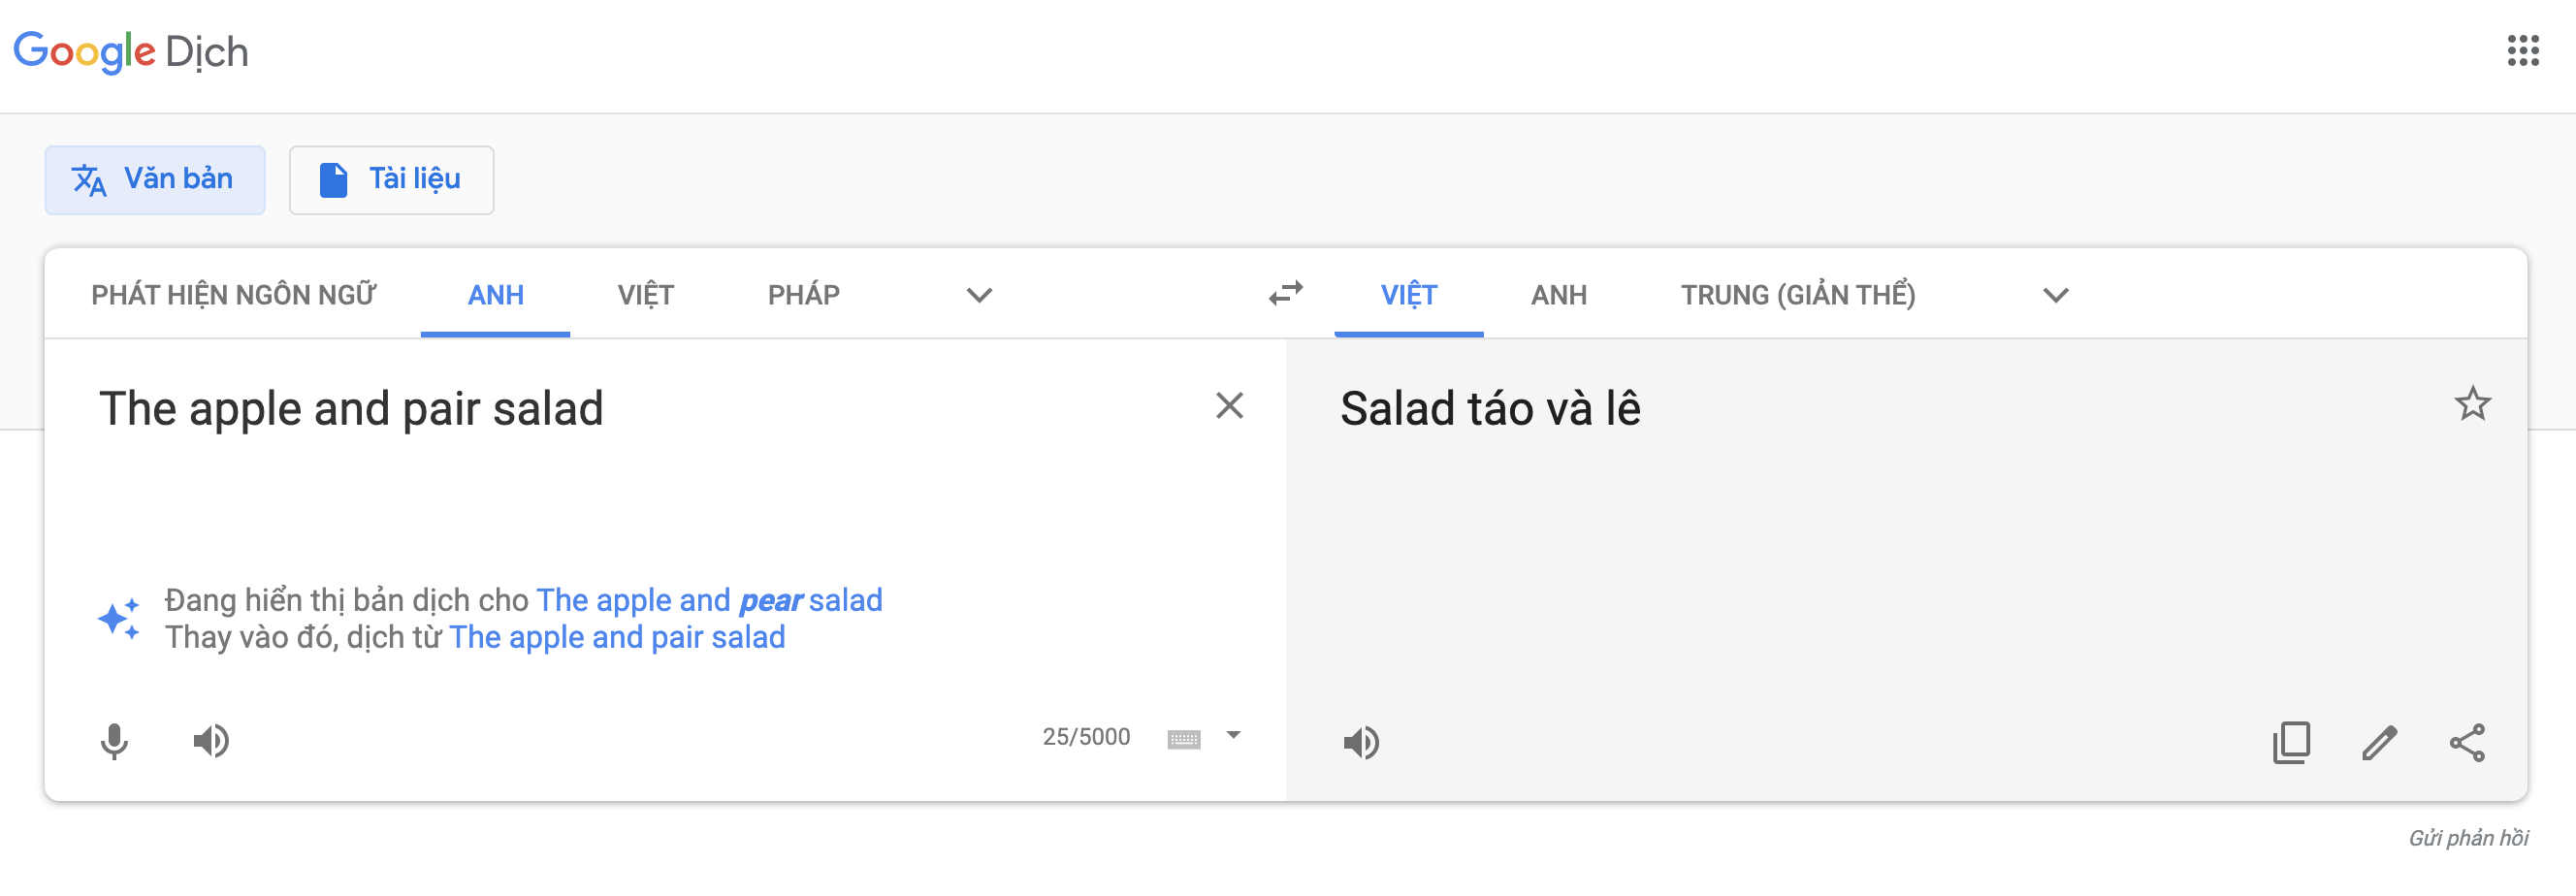
\includegraphics[width=13cm]{chapter07/figure-sec12/google-translate.png}
    \caption{Nhờ có mô hình ngôn ngữ mà Google Translate có thể nhận biết giọng nhất (các từ đồng âm) và sửa lỗi chính tả.}
    \label{fig:google-translate}
\end{figure}

\subsection{Ước lượng xác suất và mô hình n-gram}
\subsubsection{Ước lượng xác suất}
Cách đơn giản nhất để tính các xác suất là ước lượng tương đối sự xuất hiện của câu đó bằng cách đếm hết xuất hiện của câu đó trong tất cả các câu. Ví dụ:
\begin{equation}
\begin{split}
P("\text{Chúng ta không thuộc về nhau}")&=\frac{count(\text{Chúng ta không thuộc về nhau})}{count(\text{Tất cả các câu được nói/viết})}.\\
\end{split}
\end{equation}

Hoặc với xác suất likelihood thì:
\begin{equation}
\begin{split}
P(\text{nhau | chúng ta không thuộc về})&=\frac{count(\text{chúng ta không thuộc về nhau})}{count(\text{chúng ta không thuộc về})}.\\
\end{split}
\end{equation}

Tuy nhiên với cách ước lượng này thì không khả thi do thực tế có rất nhiều, vô hạn chuỗi từ/câu  và chúng ta không thể thấy đủ dữ liệu để ước lượng. 

Do đó trên thực tế, các mô hình ngôn ngữ thường dựa vào \textbf{tính chất Markov (\textit{Markov property})}: tương lai không phụ thuộc quá khứ nếu biết hiện tại, cụ thể: 
$$P(w_i|w_1,w_2,...,w_{i-1})=P(w_i|w_{i-1})$$
Ví dụ: P(nhau | chúng ta không thuộc về) = P(nhau | về).

Hay tổng quát hơn, \textbf{$k$-order Markov property} giả sử rằng từ tiếp theo xuất hiện trong chuỗi chỉ phụ thuộc vào $k$ từ trước:
$$P(w_i|w_1,w_2,...,w_{i-1})=P(w_i|w_{1:i-1-k})$$

Mặc dầu, tính chất Markov không phải là một cách tiếp cận hoàn toàn đúng và bền vững (\textit{robust}) (ví dụ: câu có chiều dài bất kỳ và có thể rất dài. Từ cuối lại có thể liên quan để các từ đầu tiên và ngoài khoảng $k$ (\textbf{long-distance dependencies}). Tuy nhiên, mô hình hoá ngôn ngữ dựa vào tính chất Markov vẫn là một cách hữu hiệu và đưa ra được một mô hình hoá mạnh với một số $k$ hợp lý.

\subsubsection{Mô hình n-gram}
Dựa trên tính chất Markov, ta có mô hình ngôn ngữ $n$-gram ($n$-gram language model): gán xác suất dựa vào $n$ từ ($n$-gram). Ý tưởng về $n$-gram khởi nguồn từ những công trình Lý thuyết thông tin (\textit{Information Theory}) của \textit{Claude Shannon} khi ông đặt câu hỏi về cho một chuỗi các ký tự thì xác suất xuất hiện (\textit{likelihood}) của từ tiếp theo là bao nhiêu.


Trường hợp đơn giản nhất là \textbf{Unigram model} hay các từ xuất hiện sau không phụ thuộc (độc lập) với các từ phía trước.
$$P(w_1w_2...w_n)\approx\prod_{i=1}^{n} P(w_i)$$

Tiếp đến là \textbf{Bigram model}: từ dự đoán phụ thuộc vào một từ trước đó.
$$P(w_i|w_1w_2...w_{i-1})\approx\prod_{i=1}^{n} P(w_i|w_{i-1})$$


\begin{figure}[H]
    \centering
    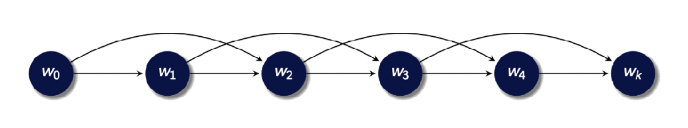
\includegraphics[width=13cm]{chapter07/figure-sec12/bigram.png}
    \caption{Bigram Language Model.}
    \label{fig:bigram}
\end{figure}

Dựa vào hình \ref{fig:bigram}, ta có thấy:
\begin{itemize}
    \item $P(w_1|w_0)=P(w_1|w_0)$
    \item $P(w_2|w_1w_0)=P(w_2|w_1)$
    \item $P(w_3|w_2w_1w_0)=P(w_3|w_2)$
    \item ...
    \item $P(w_k|w_{k-1}...w_2w_1w_0)=P(w_k|w_{k-1})$
\end{itemize}

Từ đó ta có thể tính 
\begin{equation}
\begin{split}
P(w_i|w_{i-1})&=\frac{count(w_i,w_{i-1})}{count(w_{i-1})}.\\
\end{split}
\end{equation}

Ví dụ: giả sử câu bắt đầu với <s> và kết thúc với </s>. Xét 3 câu sau:

<s> I am Sam </s>

<s> Sam I am </s>

<s> I do not like green eggs and ham </s>

Ta có:

$P(I|<s>)=\frac{2}{3}$, $P(Sam|<s>)=\frac{1}{3}$,$P(am|I)=\frac{2}{3}$, 

$P(</s>|Sam)=\frac{1}{2}$,$P(Sam|am)=\frac{1}{2}$,$P(do|I)=\frac{1}{3}$.

Đối với \textbf{Trigram model} thì: 
\begin{equation}
\begin{split}
P(w_i|w_{i-1}w_{i-2})&=\frac{count(w_i,w_{i-1},w_{i-2})}{count(w_{i-1},w_{i-2})}.\\
\end{split}
\end{equation}

Chúng ta có thể mở rộng ra cho trigram, 4-gram,... 

\begin{figure}[H]
    \centering
    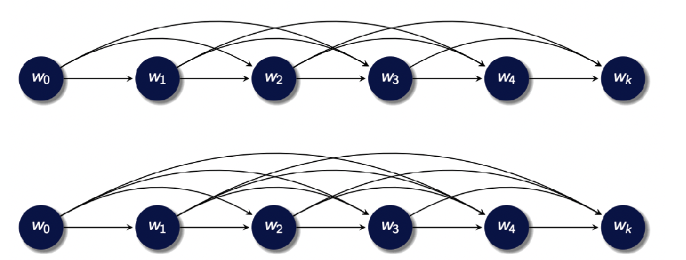
\includegraphics[width=13cm]{chapter07/figure-sec12/ngram.png}
    \caption{$n$-gram Language Model: trigram và 4-gram}
    \label{fig:ngram}
\end{figure}

\underline{Thảo luận:}

Như chúng ta đã biết, ngôn ngữ có sự phụ thuộc khoảng cách dài (\textit{long distance dependencies}). Xét câu sau: 

\begin{center}
He drives a new Audi car to his penhouse. (1)
\end{center}

Trong câu trên để mô hình cho kết quả tốt, ta phải dùng ít nhất 7-grams. Hoặc xét câu sau:
\begin{center}
The man who moves mountain begins by carrying away small stones. (2)
\end{center}    

Rõ ràng từ "begins" có likelihood phụ thuộc vào từ "man" nhưng nếu $n$ không đủ lớn thì output của mô hình ngôn ngữ sẽ không ra xác suất cao cho những câu này và ra xác suất cao cho những câu không phù hợp (có thể là dựa vào từ "mountain").

Mặt khác như $n$ quá lớn thì cũng khó để ước lượng các xác suất bởi vì thưa dữ liệu. Ví dụ với câu (1), giả sử ta dùng 7-grams thì sẽ có $|V|^7$ biến cố (với $|V|$ là lực lượng của vocabulary), với một vocabulary rất nhỏ với $|V|=10^4$ thì sẽ có tới $10^{28}$ biến cố khác nhau.

Như vậy, với việc chọn $n$ là một \textbf{bias-variance tradeoff}. Một $n$ nhỏ sẽ có một bias cao, và cao sẽ cho một varinace cao. Chúng ta có thể giải quyết vấn đề này bằng cách vẫn giữ nguyên $n$ lớn và cộng với smoothing.

\subsection{Đánh giá mô hình ngôn ngữ}
Mô hình ngôn ngữ tốt là một mô hình cho xác suất các câu tốt (phù hợp và thường xuyên xuất hiện) cao hơn các câu "không" tốt (ví dụ: không phù hợp ngữ pháp và thường xuyên xuất hiện). Vì sự phức tạp của ngôn ngữ nên việc đánh giá một mô hình ngôn ngữ A tốt hơn mô hình ngôn ngữ B là rất khó khăn.

Một cách tiếp cận là \textbf{đánh giá ngoài (\textit{extrinsic evaluation})}. Đặt hai mô hình ngôn ngữ A và B vào một công việc cụ thể. Ví dụ: kiểm tra lỗi chính tả, dịch máy,... và kiểm tra độ chính xác cho A và B theo một metric nhất định rồi cho ra kết quả so sánh.

Ví dụ: đối với kiểm tra lỗi chính tả, ta có thể kiểm tra: Có bao nhiêu từ sai chính tả được sửa lại cho đúng.

Tuy nhiên, đối với cách đánh giá này thì vô cùng tốn thời gian (có thể mấy cả tuần, tháng) nên trong thực tế ta dùng \textbf{đánh giá trong (\textit{intrinsic evaluation})}: dùng độ do \textbf{Perplexity}.

Trong lý thuyết thông tin, độ do Perplexity dùng để đo một phân bố xác suất hay một mô hình xác suất có đủ tốt để dự đoán một mẫu (\textit{sample}). Một mô hình ngôn ngữ tốt là một mô hình mà có thể dự đoán tốt trên tập dữ liệu kiểm tra (test set). Cho một corpus gồm $n$ từ $w_1,...,w_n$ và một mô hình ngôn ngữ gán xác suất cho một từ dựa vào lịch sử, Perplexity được tính như sau:
\begin{equation}
\label{chp07:eq7}
PP(p)=2^{H(p)}=2^{-\sum_{x}^{}p_x\log_2p_x}
\end{equation}
Trong đó, $H(p)$ là hàm cross-entropy của phân bố xác suất đó.

Perplexity càng nhỏ thì mô hình ngôn ngữ càng fit tốt vì việc tối thiểu hoá perplexity sẽ tương đương với tối đa hoá xác suất. Perplexity đặc thù từng corpus nên khi so sánh hai mô hình ngôn ngữ thì ta phải chọn cùng một tập unseen corpus (test set) đánh giá. 

Với một câu đủ dài ($N$ nào đó), theo định lý \textbf{\textit{Shannon-McMillan-Breiman}} ta có:
$$H(p)\approx-\frac{1}{N}log_2p(W)=-\frac{1}{N}log_2p(w_1,w_2,...,w_N)$$

Do đó ta có thể biến đổi công thức \ref{chp07:eq7} thành: 
\begin{equation} 
\begin{split}
PP(p)&=2^{-\frac{1}{N}log_2p(w_1,w_2,...,w_N)}\\
&=(2^{log_2p(w_1,w_2,...,w_N)})^{-\frac{1}{N}}\\
&=p(w_1,w_2,...,w_N)^{-\frac{1}{N}}\\
&=  \sqrt[n]{\frac{1}{p(w_1,w_2,...,w_N)}}\\
\end{split}
\end{equation}

Ví dụ: cho một chuỗi số ngẫu nhiên từ 0->9, xác suất xuất hiện của từ tiếp theo biết xác xuất suất hiện của mỗi từ là $1/10$ thì perplexity của mô hình này là:
$$PP(p)=p(w_1,w_2,...,w_N)^{\frac{1}{N}}=(\frac{1}{10}^N)^{-\frac{1}{N}}=\frac{1}{10}^{-1}=10$$

Giá trị perplexity của các mô hình ngôn ngữ N-gram khác nhau được đào tạo bằng cách sử dụng 38 triệu từ và được kiểm tra bằng cách sử dụng 1,5 triệu từ từ tập dữ liệu của The Wall Street Journal (WSJ):
\begin{table}[H]
\centering
\begin{tabular}{ |c|c|c|c| } 
 \hline
 N-gram Order & Unigram & Bigram & Trigram \\ 
  \hline
 Perplexity & 962 & 170 & 109 \\ 
 \hline
\end{tabular}
\caption{Perplexity tương ứng với các n-gram khác nhau}
\label{Perplexity}
\end{table}
 Như chúng ta đã biết, Perplexity thì mô hình ngôn ngữ càng tốtm như vậy trong ba mô hình so sánh trong bảng \ref{Perplexity} thì Trigram tốt hơn hai mô hình còn lại.
 
 Để hiểu sâu hơn về độ đo Perplexity, ta tạm gác ngôn ngữ và gán xác suất cho từ. Giả sử mô hình dự đoán kết quả của việc tung một con súc sắc. Một con xúc xắc thông thường có 6 mặt, do đó \textit{hệ số phân nhánh (branching factor)} của con xúc xắc là 6. Hệ số phân nhánh cho biết có bao nhiêu kết quả có thể xảy ra bất cứ khi nào chúng ta tung.
 
 Giả sử huấn luyện một mô hình trên con xúc xắc đều và mỗi lần tung sẽ có xác suất $\frac{1}{6}$ nhận được bất kỳ mặt nào. Sau đó, giả sử chúng ta tạo bộ thử nghiệm bằng cách tung con xúc xắc 10 lần nữa và chúng ta thu được chuỗi kết quả  T = \{1, 2, 3, 4, 5, 6, 1, 2, 3, 4\}. Giá trị perplexity của mô hình này trên test data là bao nhiêu?
 
 $$PP(p)=\frac{1}{(\frac{1}{6}^{10})^{\frac{1}{10}}}=6$$
 Như vậy giá trị perplexity chính là \textbf{\textit{hệ số phân nhánh (branching factor)}}.
 
 Bây giờ, hãy tưởng tượng rằng chúng ta có một con xúc xắc không đều, mặt số 6 có xác suất xuất hiện là $\frac{7}{12}$ và tất cả các mặt còn lại có xác suất là $\frac{1}{12}$. Chúng tôi huấn luyện một mô hình và sau đó tạo một test set T bằng cách tung con súc sắc $12$ lần: thì được mặt số $6$ trên $7$ tung và các số khác trên $5$ tung còn lại. Giá trị perplexity: 
 
  $$PP(p)=\frac{1}{((\frac{7}{12})^{7}*(\frac{1}{12})^{5})^{\frac{1}{12}}}=3.9\approx 4$$
  
  Giá trị perplexity lúc này thấp hơn, mô hình biết được sự xuất hiện của mặt số 6 nhiều hơn các mặt còn lại nên nó không "bất ngờ" lắm hay mô hình lúc này dự đoán tốt hơn. Hệ số phân nhánh lúc này vẫn là 6 (có 6 mặt có thể xuất hiện) nhưng \textbf{hệ số phân nhánh có trọng số (weighted branching factor)} xấp xỉ 4. Ta có thể nói là mô hình không chắc chắc trong việc dự đoán từ 4 từ tiếp theo (thay vì 6 
 từ như hệ số phân nhánh ban đầu).
 
 Rõ ràng hơn, giả sử với một con xúc xắc có không đều có xác suất xuất hiện mặt số 6 là 99\% và các mặt khác chỉ $\frac{1}{500}$ trong 100 lần thử thì:
  $$PP(p)=\frac{1}{((\frac{99}{100})^{99}*(\frac{1}{500})^{1})^{\frac{1}{100}}}=1.07\approx 1$$
  
  Hệ số phân nhánh khi này vẫn là 6 nhưng hệ số phân nhánh có trọng số chỉ là 1. Có thể nói mô hình gần như chắc chắn mặt xuất hiện khi tung là mặt số 6 mặc dầu về lý thuyết các mặt khác vẫn có thể xuất hiện. 
  
  Trở lại với các mô hình ngôn ngữ và việc gắn xác suất cho từ, nếu chúng ta có một mô hình ngôn ngữ đang cố gắng dự đoán từ tiếp theo, thì hệ số phân nhánh đơn giản là số lượng từ có thể: bằng kích thước của từ vựng. Tuy nhiên bằng việc gán xác suất một cách "hợp lý" thì ta có thể thu giảm số này.
  
  Ví dụ: nếu ta có giá trị perplexity là 4, thì đó \textit{hệ số phân nhánh trung bình}. Khi cố gắng đoán từ tiếp theo, mô hình không chắc chắn như thể phải chọn giữa 4 từ khác nhau.
  
  \subsection{Làm trơn mô hình ngôn ngữ}
  Mô hình ngôn ngữ $N$-grams hoạt động tốt nếu tập kiểm tra giống phân bố với tập huấn luyện. Tuy nhiên trên thực tế thì các nhiều câu, chuỗi từ không biết trước và không có trong tập huấn luyện nhưng lại xuất hiện trong tập kiểm tra. Điều này làm cho việc gán xác suất bằng $0$ cho các câu này (gán xác suất bằng $0$ cho biến cố từ xuất hiện tiếp theo $w_k$ nào đó và tính chất nhân tính của việc tính toán chuỗi xác suất câu). 
  
  Ví dụ: ta có tập huấn luyện gồm các câu sau:
  \begin{itemize}
      \item Chúng ta không thuộc về nhau.
      \item Chúng ta không thuộc về đâu.
      \item Chúng ta không thuộc về đây.
  \end{itemize}
  
  Nhưng tập kiểm tra thì:
  \begin{itemize}
  \item Chúng ta không thuộc về đó.
  \item Chúng ta không thuộc về thành phố.
  \end{itemize}
  
  Khi đó giá trị perplexity không thể tính được vì không thể chia cho xác suất $0$ hay nói cách khác ta có perplexity bằng vô hạn - mô hình ngôn ngữ cực kỳ tệ. 
  
Xét mô hình Bigram, ta có:
\begin{equation}
\begin{split}
P(w_i|w_{i-1})&=\frac{count(w_{i-1},w_i)}{count(w_{i-1})}.\\
\end{split}
\end{equation}

Giả sử chuỗi $<w_i,w_{i-1}>$ không xuất hiện trong tập huấn luyện thì $count(w_{i-1},w_i)=0$ dẫn tới $P(w_i|w_{i-1})=0$. Ước lượng này còn được gọi là \textbf{uớc lượng hợp lý cực đại (Maximum likelihood estimation - MLE)}.

Giải quyết tình trạng xác đó ta dùng kỹ thuật \textit{làm trơn (smoothing)} mô hình ngôn ngữ. Một trong những kỹ thuật làm trơn thường dùng nhất là \textbf{làm trơn Laplace (Laplace smoothing)}: cộng $1$ cho tất cả các từ trong tập từ vựng. 
\begin{equation}
\label{chp07:eq10}
\begin{split}
P(w_i|w_{i-1})&=\frac{count(w_{i-1},w_i)+1}{count(w_{i-1})+|V|}.\\
\end{split}
\end{equation}

Trong đó $|V|$ là kích thước tập từ vượng, ước lượng này còn được gọi là \textbf{ước lượng add-1 (add-1 estimation)}. Tổng quát hơn ta có \textbf{ước lượng add-$\alpha$ (add-$\alpha$ estimation)} với $0<\alpha \leq 1$:
\begin{equation}
\label{chp07:eq11}
\begin{split}
P(w_i|w_{i-1})&=\frac{count(w_{i-1},w_i)+\alpha}{count(w_{i-1})+\alpha|V|}.\\
\end{split}
\end{equation}

Với kỹ thuật làm trơn add-1 trong công thức \ref{chp07:eq10}, ta có thể hoàn nguyên lại số (count) sự hiện của các từ:
\begin{equation}
\begin{split}
count*(w_{i-1},w_i)&=\frac{(count(w_{i-1},w_i)+1)*count(w_{i-1})}{count(w_{i-1})+|V|}.\\
\end{split}
\end{equation}

\begin{figure}[H]
    \centering
    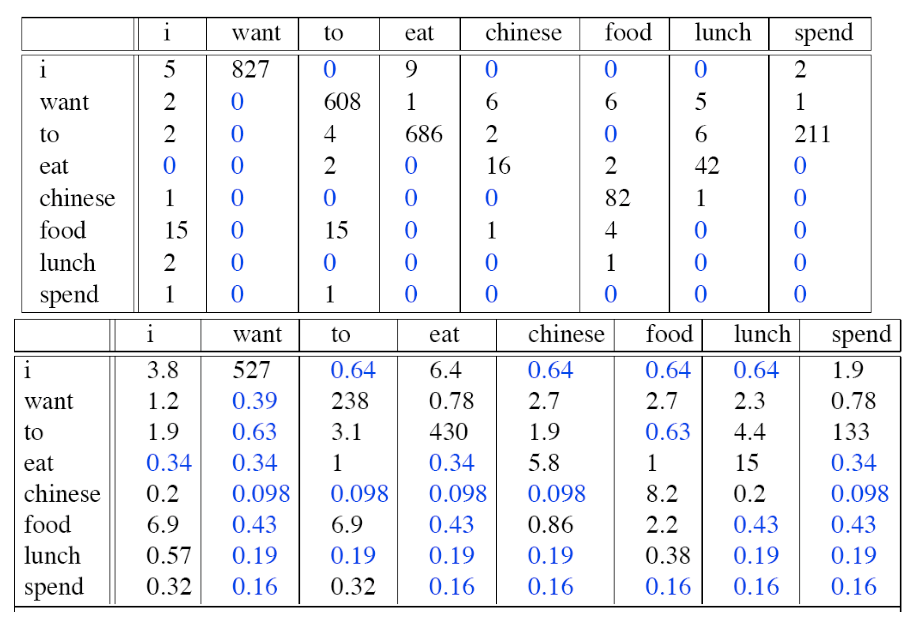
\includegraphics[width=10.5cm]{chapter07/figure-sec12/smoothing.png}
    \caption{So sánh count của bigram: bảng phía trên xuất hiện nhiều count bằng $0$. Bảng dưới sau khi được làm trơn bằng ước lượng add-1 và hoàn nguyên lại count.}
    \label{fig:smoothing}
\end{figure}

Một trường hợp khác là mô hình $N$-gram nhưng ta không quan sát được đủ $N$ khi đó một kỹ thuật làm trơn khác thuờng được dùng là \textbf{\textit{back-off}}: tính toán các ước lượng dựa trên $(N-1)$-gram:
\begin{equation}
\label{chp07:eq13}
\begin{split}
P(w_{i+1}|w_{i-k:i})&=\beta*\frac{count(w_{i-k:i+1})}{count(w_{i-k:i})}+(1-\beta)P(w_{i+1}|w_{i-(k-1):i}).\\
\end{split}
\end{equation}

Phép làm trơn trong công thức \ref{chp07:eq13} còn gọi là \textbf{\textit{Jelinek Mercer interpolated smoothing}}.

Một cách tiếp cận khác là \textbf{\textit{Nội suy tuyến tính (Linear Interpolation)}}: trộn lẫn giữa unigram, bigram và trigram. Kí hiệu $\hat{P}$ là xác suất được làm trơn, ta có:
$$\hat{P}(w_n|w_{n-1}w_{n-2})=\lambda_1 P(w_n|w_{n-1}w_{n-2})+\lambda_2 P(w_n|w_{n-1})+\lambda_3 P(w_n)$$

Trong đó, $\lambda_1 \geq 0,\lambda_2 \geq 0,\lambda_3 \geq 0$ và $\lambda_1 +\lambda_2 + \lambda_3 =1$.
